\documentclass[a4paper,10pt]{article}
\usepackage[utf8]{inputenc}
\usepackage{amssymb}
\usepackage{amsfonts}
\usepackage{amsmath}
\usepackage{enumerate}
\setlength{\parindent}{0pt}
\usepackage[margin=1in]{geometry}

\usepackage{graphicx}
\graphicspath{ {./images/} }

\usepackage{listings}
\usepackage{color}

\definecolor{dkgreen}{rgb}{0,0.6,0}
\definecolor{gray}{rgb}{0.5,0.5,0.5}
\definecolor{mauve}{rgb}{0.58,0,0.82}

\lstset{frame=tb,
  language=C++,
  aboveskip=3mm,
  belowskip=3mm,
  showstringspaces=false,
  columns=flexible,
  basicstyle={\small\ttfamily},
  numbers=none,
  numberstyle=\tiny\color{gray},
  keywordstyle=\color{blue},
  commentstyle=\color{dkgreen},
  stringstyle=\color{mauve},
  breaklines=true,
  breakatwhitespace=true,
  tabsize=3
}
\begin{document}

Jason Qiu

CS 385 Homework Assignment $\#4$

\emph{I pledge my honor that I have abided by the Stevens Honor System.}
\begin{enumerate}
\item Instead of reversing \verb|L1| when copying to \verb|L2|, simply copy \verb|L1| into \verb|L2| without changing order.

\item \begin{enumerate}[Step 1.]
	\item Because $72 < 93$, no need to swap.
	\item Divide $n = 72$ until we get 1, while multiplying $m = 93$:

	\centerline{
	\begin{tabular}{c|c}
	$n$ & $m$ \\
	\hline
	72 & 93\\
	36 & 186\\
	18 & 372\\
	9 & 744\\
	4 & 1488\\
	2 & 2976\\
	1 & 5952
	\end{tabular}
	}
	
	\item Strike out evens:
	
	\centerline{
	\begin{tabular}{c|c}
	$n$ & $m$ \\
	\hline
	72 & *\\
	36 & *\\
	18 & *\\
	9 & 744\\
	4 & *\\
	2 & *\\
	1 & 5952
	\end{tabular}
	}
	
	\item Add $m$'s up: $72 \cdot 93 = 744 + 5952 = \boxed{6696}$

\end{enumerate}

\item \begin{enumerate}[(a)]
	\item Quicksort's worst cases are when each recursive step it selects a pivot that's either the lowest or highest value element in the array. So, an already sorted or reverse-sorted array, or an array whose values are all the same (although that's the same as already sorted).
	\item In the worst case, each recursive step of Quicksort sorts either the largest or smallest element and will generate an unsorted array of size $n-1$ behind or ahead of it. This means it takes $T(n) = T(n-1) + \Theta (n), T(0) = 0$ time. Therefore, it will take $\Theta(n^2)$ time in the worst case.

\end{enumerate}

\item \begin{enumerate}[Step 1.]
	\item Divide each item into two-digit multiplications: $2205 \cdot 1132 = (22 \cdot 100 + 05) \cdot (11 \cdot 100 + 32) = (22 \cdot 11) \cdot 100^2 + (22 \cdot 32 + 05 \cdot 11) \cdot 100 + (05 \cdot 32)$
	\item Rewrite as product of $c_2, c_1, c_0$ and powers of 10: $(22 \cdot 11) \cdot 100^2 + (22 \cdot 32 + 05 \cdot 11) \cdot 100 + (05 \cdot 32) = c_2 \cdot 10^4 + c_1 + 10^2 + c_0$
	
	\item Calculate $c_2 = 22 \cdot 11$ by dividing each item into one-digit multiplications: $22 \cdot 11 = (2 \cdot 10 + 2) \cdot (1 \cdot 10 + 1) = (2 \cdot 1) \cdot 10^2 + (2 \cdot 1 + 2 \cdot 1) \cdot 10 + (2 \cdot 1)$

	\item Rewrite as product of $x_2, x_1, x_0$: $(2 \cdot 1) \cdot 10^2 + (2 \cdot 1 + 2 \cdot 1) \cdot 10 + (2 \cdot 1) = x_2 \cdot 10^2 + x_1 \cdot 10 + x_0$
	\item Calculate $x_2 = 2 \cdot 1 = 2$
	\item Calculate $x_0 = 2 \cdot 1 = 2$
	\item Calculate $x_1 = (2 + 2)(1 + 1) - 2 - 2 = 8 - 2 - 2 = 4$
	\item Substitute $x_2, x_1, x_0$: $c_2 = x_2 \cdot 10^2 + x_1 \cdot 10 + x_0 = 2 \cdot 10^2 + 4 \cdot 10 + 2 = 200 + 40 + 2 = 242$
	
	\item Calculate $c_0 = 05 \cdot 32$ by dividing each item into one-digit multiplications: $05 \cdot 32 = (0 \cdot 10 + 5) \cdot (3 \cdot 10 + 2) = (0 \cdot 3) \cdot 10^2 + (0 \cdot 2 + 3 \cdot 5) \cdot 10 + (5 \cdot 2)$
	\item Rewrite as product of $y_2, y_1, y_0$: $(0 \cdot 3) \cdot 10^2 + (0 \cdot 2 + 3 \cdot 5) \cdot 10 + (5 \cdot 2) = y_2 \cdot 10^2 + y_1 \cdot 10 + y_0$
	\item Calculate $y_2 = 0 \cdot 5 = 0$
	\item Calculate $y_0 = 5 \cdot 2 = 10$
	\item Calculate $y_1 = (0 + 5)(3 + 2) - y_2 - y_0 = 25 - 10 = 15$
	\item Substitute $y_2, y_1, y_0$: $c_0 = 0 \cdot 10^2 + 15 \cdot 10 + 10 = 150 + 10 = 160$
	
	\item Calculate $c_1 = (22 + 05)(11+32) - c_2 - c_0 = (27 \cdot 43) - 242 - 160$
	\item Calculate $27 \cdot 43$ by dividing each item into one-digit multiplications: $22 \cdot 43 = (2 \cdot 10 + 7) \cdot (4 \cdot 10 + 3) = (2 \cdot 4) \cdot 10^2 + (2 \cdot 3 + 4 \cdot 7) \cdot 10 + (7 \cdot 3)$
	\item Rewrite as product of $z_2, z_1, z_0$: $(2 \cdot 4) \cdot 10^2 + (2 \cdot 3 + 4 \cdot 7) \cdot 10 + (7 \cdot 3) = z_2 \cdot 10^2 + z_1 \cdot 10 + z_0$
	\item Calculate $z_2 = 2 \cdot 4 = 8$
	\item Calculate $z_0 = 7 \cdot 3 = 21$
	\item Calculate $z_1 = (2+7)(4+3) - z_2 - z_0 = 63 - 8 - 21 = 34$
	\item Substitute $z_2, z_1, z_0$: $27 \cdot 43 = z_2 \cdot 10^2 + z_1 \cdot 10 + z_0 = 8 \cdot 10^2 + 34 \cdot 10 + 21 = 800 + 340 + 21 = 1161$
	
	\item Substitute to find $c_1 = 1161 - 242 - 160 = 759$
	\item Substitute $c_2, c_1, c_0$: $2205 \cdot 1132 = c_2 \cdot 10^4 + c_1 + 10^2 + c_0 = 242 \cdot 10000 + 759 \cdot 100 + 160 = 2420000 + 75900 + 160 = \boxed{2,496,060}$

\end{enumerate}

\item \ 

\centerline{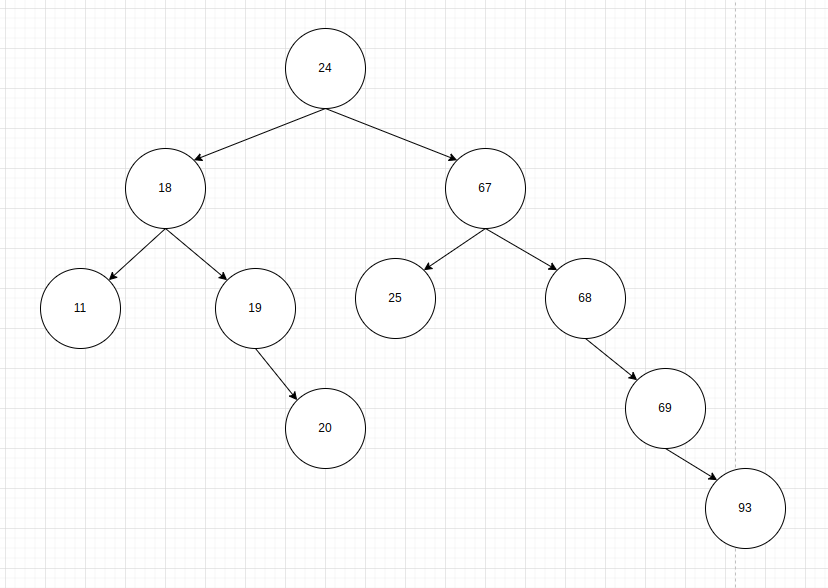
\includegraphics[scale=0.5]{fig1}}

\item \begin{enumerate}[(a)]
	\item 10, 8, 5, 3, 5, 2, 1, 7, 1, 6
	
	\item 3, 5, 5, 8, 1, 2, 10, 1, 7, 6
	
	\item 3, 5, 5, 1, 2, 8, 1, 6, 7, 10
	
	\item 4 internal nodes
	
	\item 5 leaves
	
	\item Maximum width of 4
	
	\item Height is 3
	
	\item Diameter of 5

\end{enumerate}

\item \begin{enumerate}[(a)]
	\item $\Theta(n^{\log_4{2}}) = \Theta (n^{\frac{1}{2}})$
	\item $\Theta(n^{\frac{1}{2}}\log_4{n})$
	\item $\Theta(n)$
	\item $\Theta(n^2)$
	\item $\Theta(n^3)$
\end{enumerate}

\item \begin{enumerate}[(a)]
	\item The following block of code creates a recursive call 6 times:
	\begin{lstlisting}
for(int i = 1; i <= 6; i++) {
    temp += function(n / 3);
}
	\end{lstlisting}
	Then, the next block runs in $\Theta(n^{3/2})$
	\begin{lstlisting}
for(int i = 1; i <= n; i++) {
	for(int j = 1; j * j <= n; j++) {
		temp++;
    }
}
	\end{lstlisting}
	
	So the overall runtime is $T(n) = 6T(\frac{n}{3}) + \Theta(n^{\frac{3}{2}})$.
	\item $T(n)$ is in $\Theta(n^{\log_3{6}}) \approx \Theta(n^{1.63})$

\end{enumerate}
\end{enumerate}
\end{document}